
    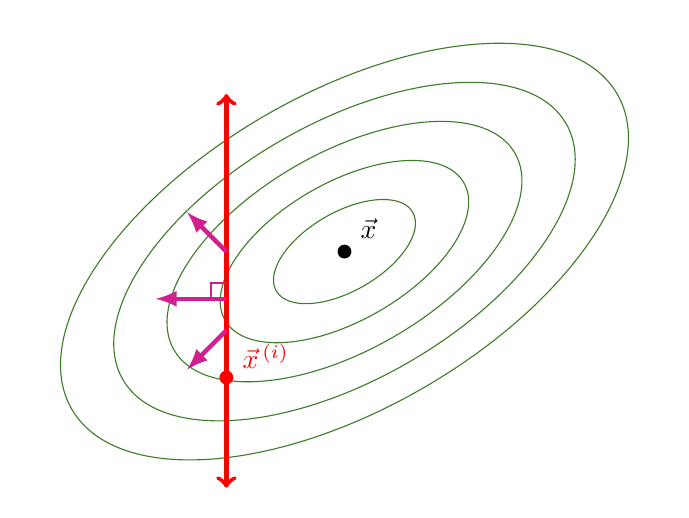
\begin{tikzpicture}
        \foreach \size in {1, 1.75, ..., 4} {
            \draw[OliveGreen, scale=\size, rotate=30] (0,0) ellipse (1cm and .5cm);
        };
        \node[circle, inner sep=0, minimum size=5pt,fill, label={30:$\vec{x}$}]() at (0,0){};


        \node[ red, circle, inner sep=0, minimum size=5pt, fill,
        label={[red, xshift=5mm, yshift=-1mm]$\vec{x}^{\,(i)}$}
        ] () at (-1.5, -1.6){};

        \draw[<->, red, ultra thick] (-1.5, -3) -- (-1.5, 2);

        \draw[->,>=latex, VioletRed, ultra thick] (-1.5, -.6) -- (-2.4, -.6);
        \draw[->,>=latex, VioletRed, ultra thick] (-1.5, -1) -- (-2, -1.5);
        \draw[->,>=latex, VioletRed, ultra thick] (-1.5, 0) -- (-2, .5);
        \draw[VioletRed, thick] (-1.7, -.6) |- (-1.5, -.4);
    \end{tikzpicture}
